\documentclass[border=10pt]{standalone}

\usepackage{tikz}
\usepackage{tikzsymbols}
\usetikzlibrary{calc,patterns,shapes.geometric}

\def\centerarc[#1](#2)(#3:#4:#5){\draw[#1] ($(#2)+({#5*cos(#3)},{#5*sin(#3)})$) arc (#3:#4:#5);}

\begin{document}
	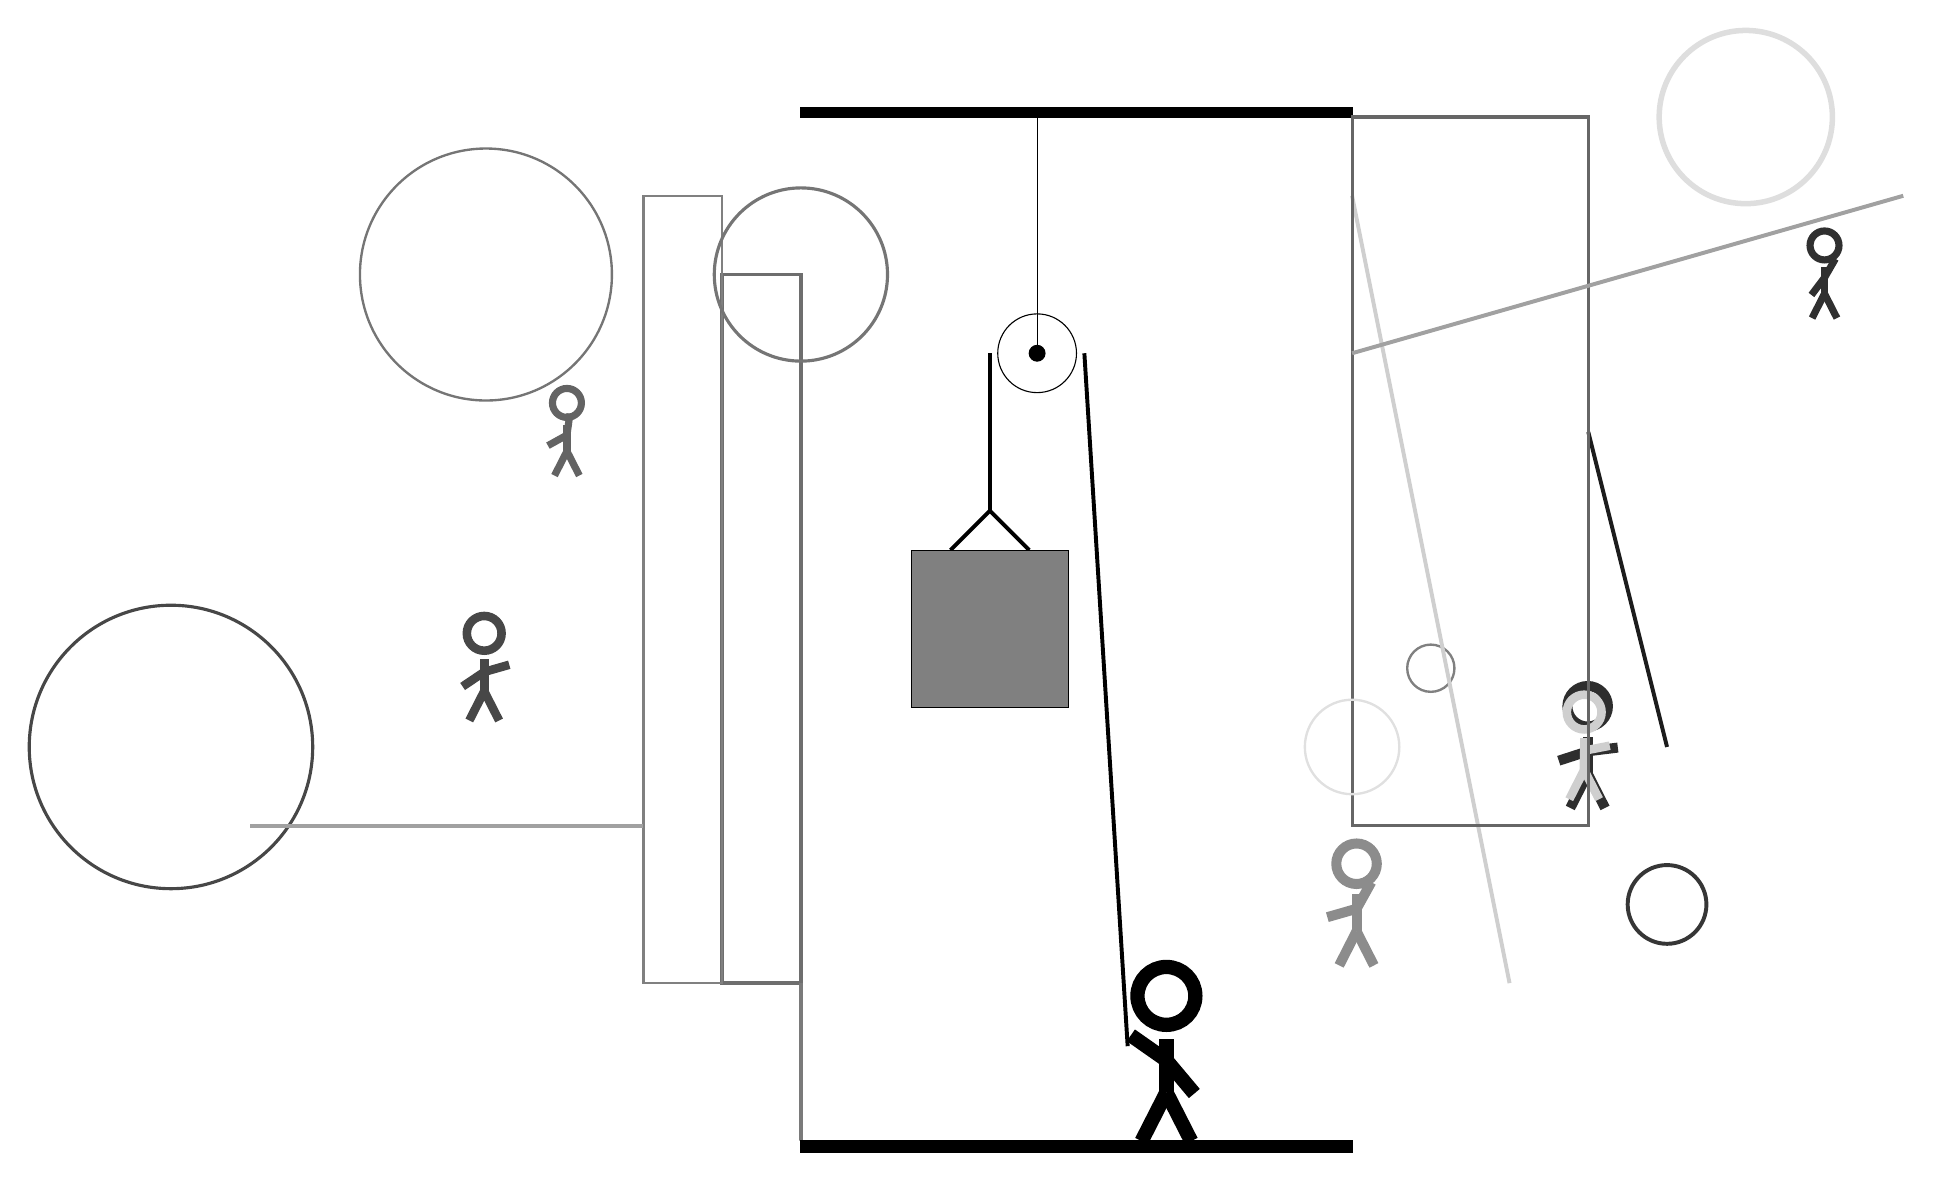
\begin{tikzpicture}
		%%%%% START %%%%%
		
		\draw[fill=black] (-2, 10) rectangle (5, 10.125);
		
		\draw (1, 7) circle (0.5);
		\draw[fill=black] (1, 7) circle (0.1);
		\draw (1, 10) -- (1, 7);
		
		\node[line width=0.3mm, color=black!45] at (5, 0) {\Strichmaxerl[7][16][61]};
		
		\draw[line width=0.5mm, color=black!89](9, 2) -- (8, 6);
		\draw[line width=0.5mm, color=black!57] (-3, 8) rectangle (-2, -1);
		\draw [line width=0.7mm, color=black!13](10, 10) circle (1.1);
		\draw [line width=0.3mm, color=black!50](6, 3) circle (0.3);
		\node[line width=0.6mm, color=black!72] at (-6, 3) {\Strichmaxerl[6][34][16]};
		\draw[line width=0.3mm, color=black!50] (-4, -1) rectangle (-3, 9);
		\draw[line width=0.5mm, color=black!19](7, -1) -- (5, 9);
		\node[line width=0.7mm, color=black!81] at (11, 8) {\Strichmaxerl[5][53][60]};
		\node[line width=0.7mm, color=black!82] at (8, 2) {\Strichmaxerl[7][18][7]};
		
		\draw [line width=0.4mm, color=black!72](-10, 2) circle (1.8);
		
		\draw[line width=0.6mm, color=black!52] (-2, -1) rectangle (-2, -3);
		\draw [line width=0.4mm, color=black!54](-2, 8) circle (1.1);
		
		\draw [line width=0.3mm, color=black!54](-6, 8) circle (1.6);
		\node[line width=0.3mm, color=black!19] at (8, 2) {\Strichmaxerl[6][89][11]};
		\draw[line width=0.4mm, color=black!60] (5, 1) rectangle (8, 10);
		\draw [line width=0.5mm, color=black!79](9, 0) circle (0.5);
		
		\draw [line width=0.3mm, color=black!12](5, 2) circle (0.6);
		\draw[line width=0.5mm, color=black!37](-4, 1) -- (-9, 1);
		\draw[line width=0.5mm, color=black!37](5, 7) -- (12, 9);
		\node[line width=0.7mm, color=black!61] at (-5, 6) {\Strichmaxerl[5][29][82]};
		
		\draw[line width=0.5mm] (-0.1, 4.5) -- (0.4, 5.0) -- (0.9, 4.5);
		\draw[fill=black!50] (-0.6, 4.5) rectangle (1.4, 2.5);
		
		\draw[line width=0.5mm] (0.4, 7) -- (0.4, 5.0);
		\centerarc[line width=0.5mm](1, 7)(0:180:0.6);
		\draw[line width=0.5mm](1.6, 7) -- (2.15, -1.8);
		
		\node at (2.6, -1.9) {\Strichmaxerl[10][-35][-50]};
		
		\draw[fill=black] (-2, -3) rectangle (5, -3.15);
		
		%%%%% END %%%%%
	\end{tikzpicture}
\end{document}